\section{Web portal deployment}

As a final step, the models created in this project were exposed using the Gradio framework, which exposes web forms using HTTP tunnelling.

We first abstracted the consumption of the models by setting up a production area in our project and creating a consumption API for each model, which, when given a single example, will return the result from the model. Although not used, we also created functionality to submit multiple lines and get a response for each in return.

We then created a Gradio application that creates a simple form to allow the user to input the data for the example, submit it, and view the results from the three models. Gradio also gives the functionality to save the results in a file.

\begin{figure}[H]
	\centering
	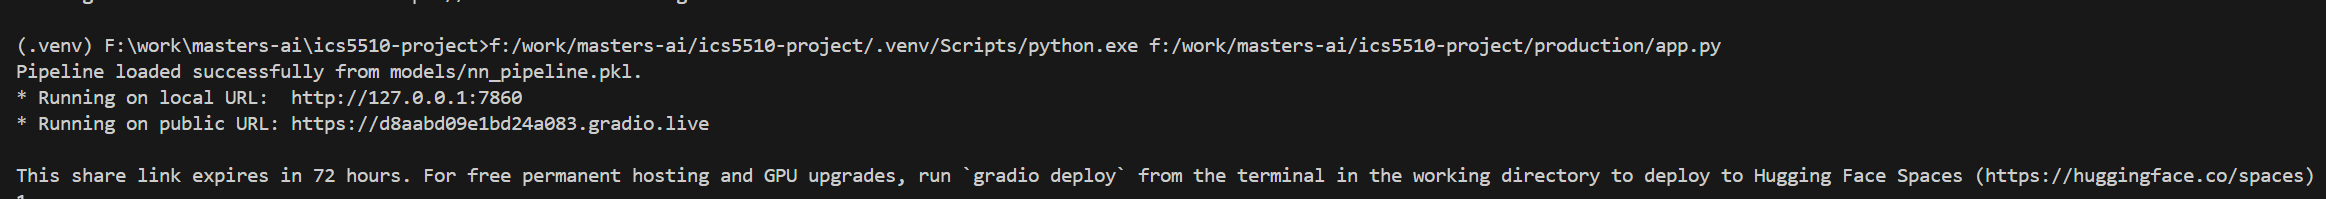
\includegraphics[width=0.9\linewidth]{F:/work/masters-ai/ics5510-project/doc/img/gradio-app-deployed}
	\caption{The Gradio application running in VSCode.}
	\label{fig:gradio-app-deployed}
\end{figure}

We tested the application locally to ensure proper functionality. Gradio also exposes the form through a remote URL that uses tunnelling to consume the app that is running locally. This URL was captured and used in a simple HTML file from GitHub as a GitHub page.


\begin{figure}[H]
	\centering
	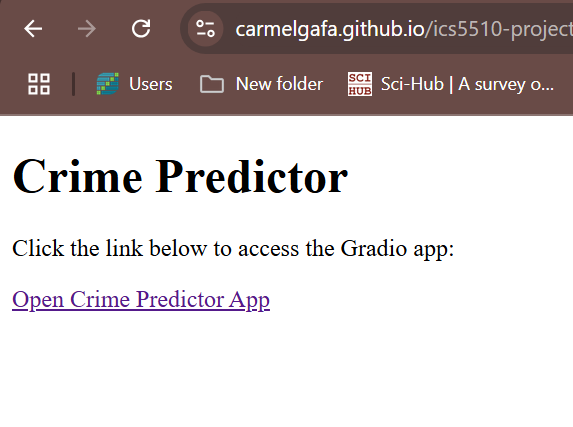
\includegraphics[width=0.7\linewidth]{img/gradio-github-page}
	\caption{GitHub page to access the Gradio app. URL: https://carmelgafa.github.io/ics5510-project/}
	\label{fig:gradio-github-page}
\end{figure}


It is important to note that Gradio’s remote URL and tunnel remain active for only 72 hours, emphasizing that this setup is intended solely as a demonstration of the system’s capabilities rather than as a production-ready solution.

\begin{figure}[H]
	\centering
	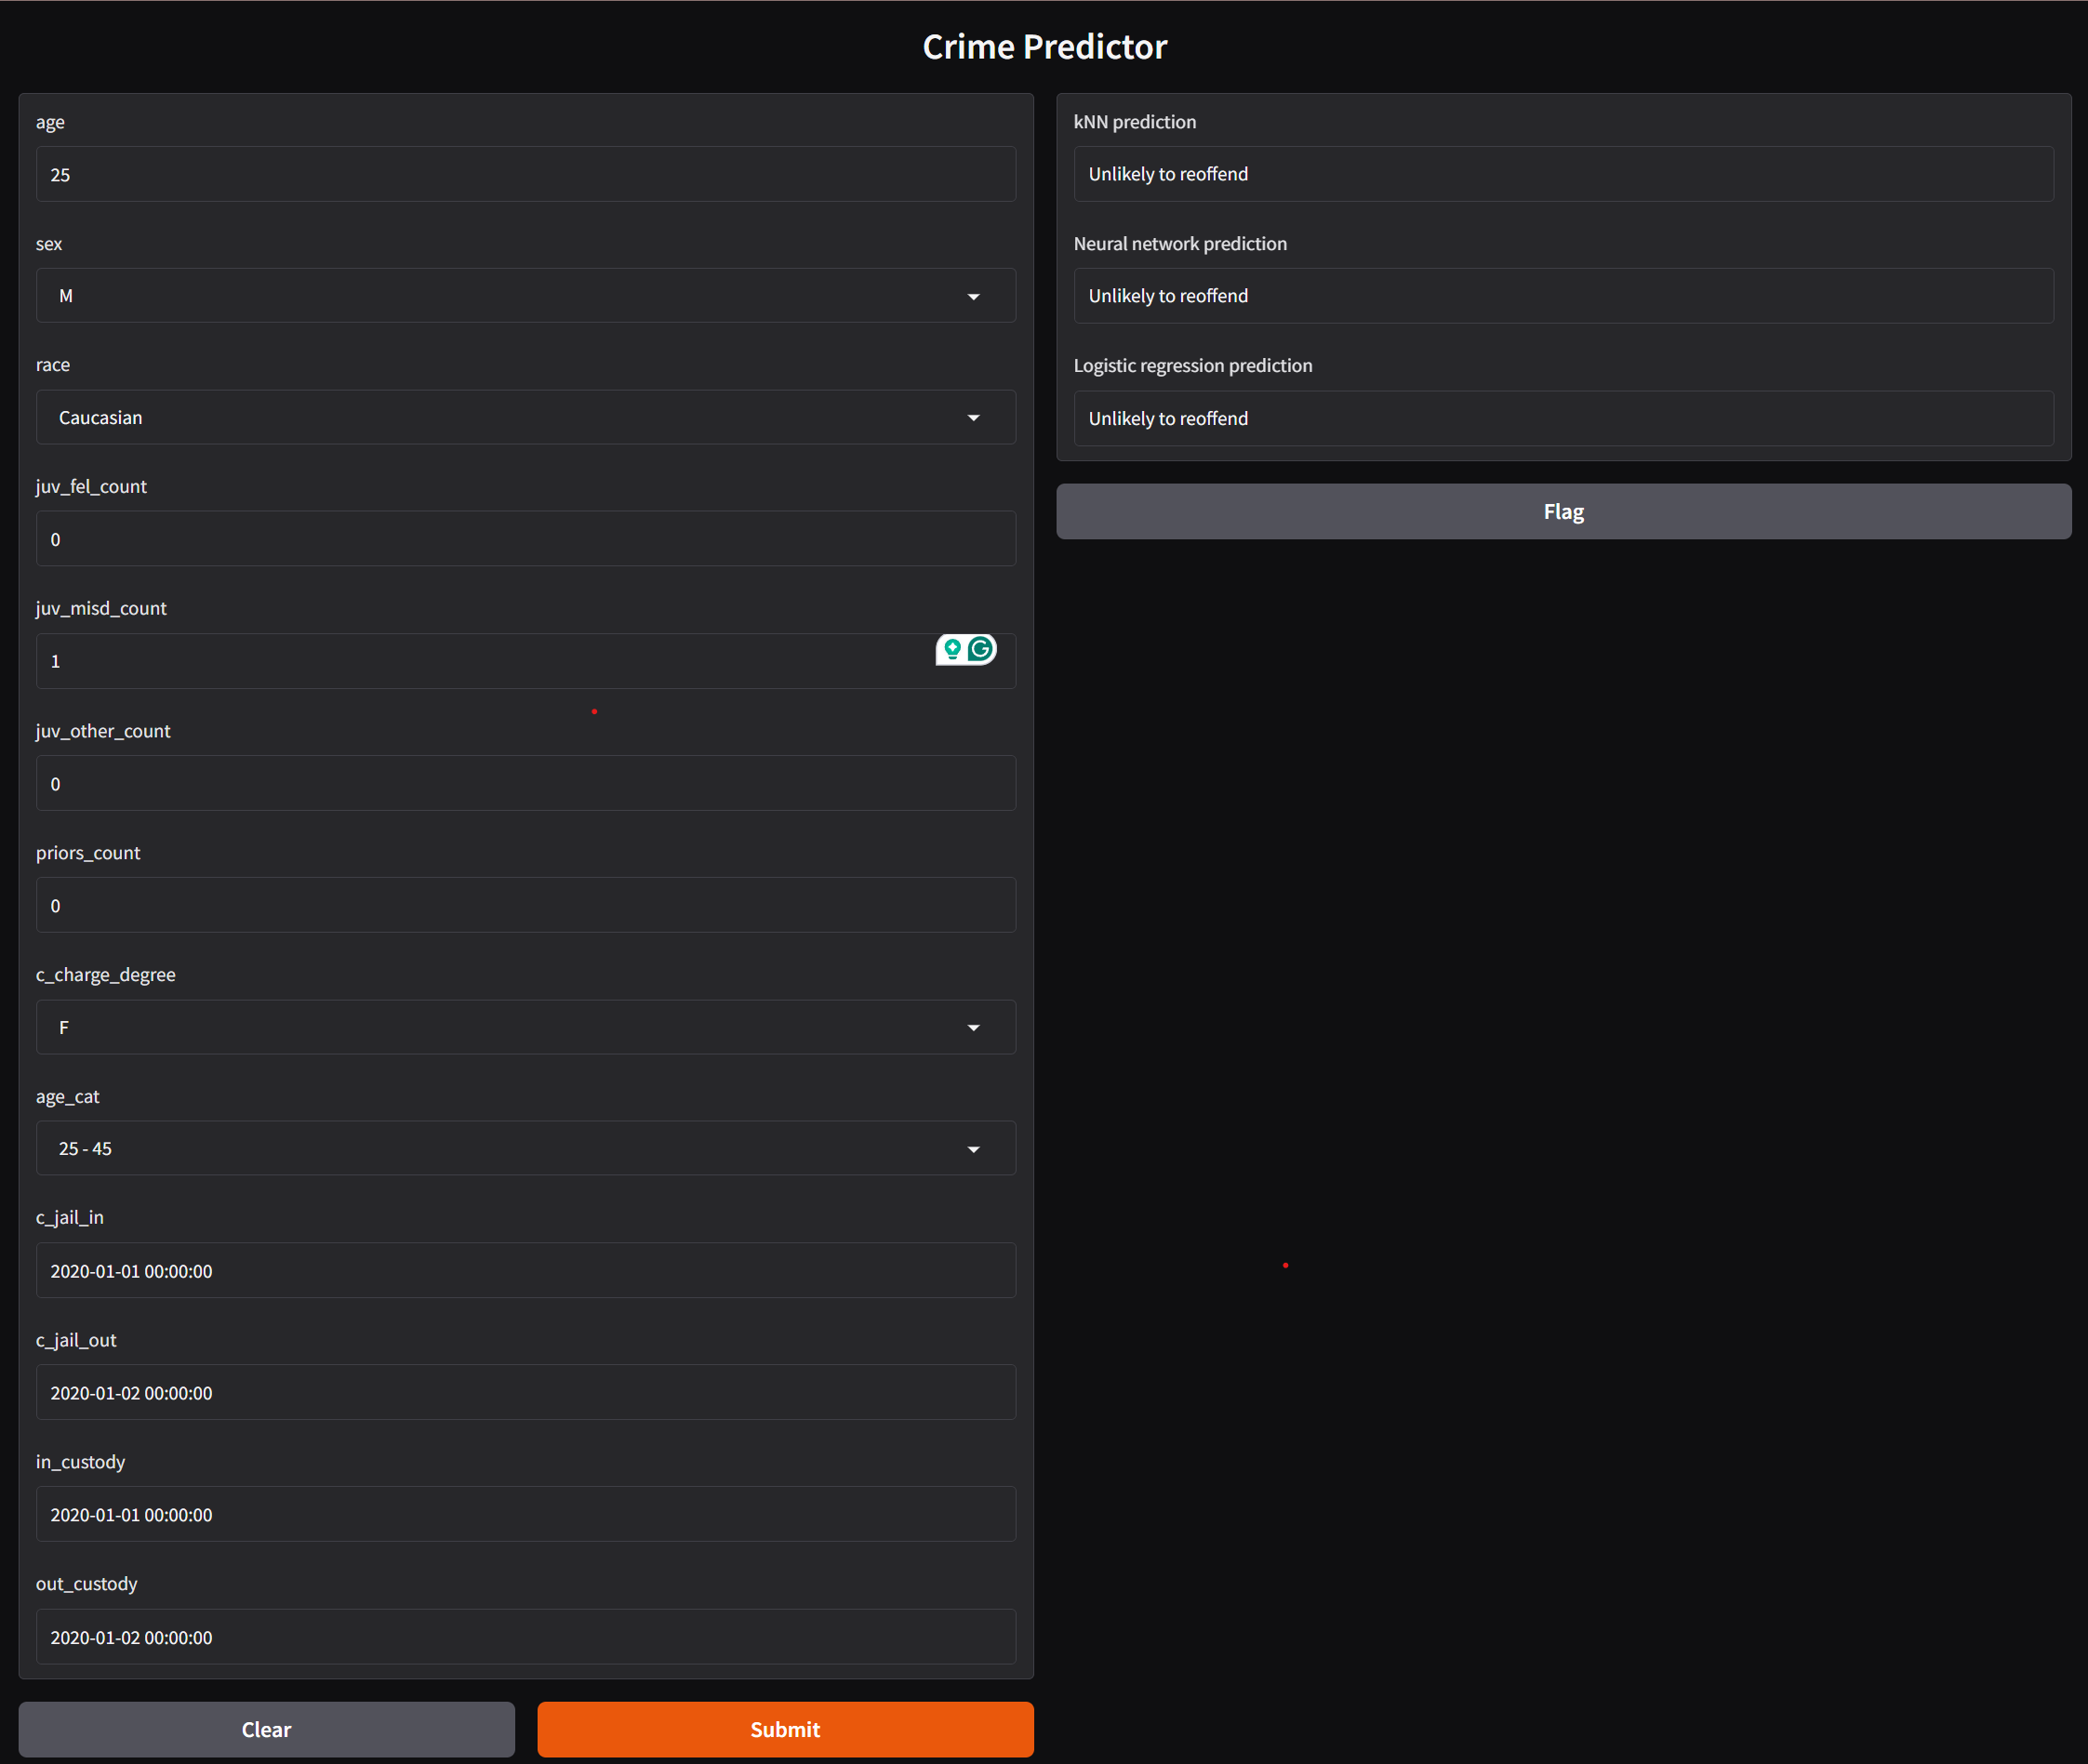
\includegraphics[width=0.7\linewidth]{img/gradio-app-page}
	\caption{Gradio app form showing the results from the three ML models.}
	\label{fig:gradio-app-page}
\end{figure}




